Der geringe Eingangswiderstand der Schaltung nach Abbildung \ref{fig:schaltplan_linearverstaerker} ist in manchen Anwendungen, wie Messungen an hochohmigen Spannungsquellen, unvorteilhaft.

In diesen Fällen kann ein sogenannter Elektrometerverstärker nach Abbildung \ref{fig:schaltplan_elektrometerverstaerker} verwendet werden, der zwar auch invertierend gegengekoppelt ist, jedoch liegt die Eingangsspannung $U_1$ an den nicht-invertierten Eingang an. 

Dies führt zu einem Eingangswiderstand $r_\text{e}=\infty$ bei idealen Operationsverstärkern und $r_\text{e}\approx 2r_{\text{gl}}$ für einen realen Operationsverstärker, wobei $r_{\text{gl}}$ der Gleichtakteingangswiderstand ist und typischerweise in der Größenordnung von 20G$\Omega$ liegt.
\begin{figure}[H]
\centering
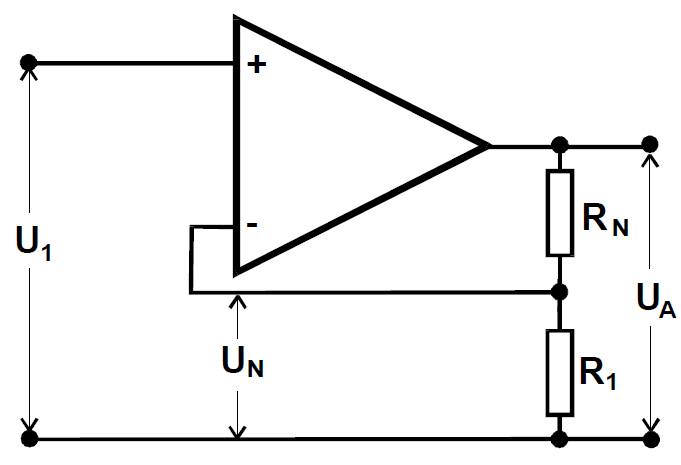
\includegraphics[width=9cm]{images/schaltplan_elektrometerverstaerker.png}
\caption{Schaltplan eines Elektrometerverstärkers. [1]}
\label{fig:schaltplan_elektrometerverstaerker}
\end{figure}
Es ergibt sich eine Verstärkung
\begin{align}
V'=\frac{R_\text{N}+R_1}{R_1}
\end{align}
des Elektrometerverstärkers bei idealen Operationsverstärkern.

Sollen kleine Ströme ohne großen Spannungsabfall gemessen werden, so wird ein Linearverstärker mit sehr geringem Eingangswiderstand $r_\text{e}$ benötigt. 

Der in Abbildung \ref{fig:schaltplan_linearverstaerker} dargestellte Linearverstärker besitzt in erster Ordnung den Eingangswiderstand $R_1$. Es liegt daher nahe, den Eingangswiderstand zu $R_1=0$ wählen. Ein solches Amp$\grave{\text{e}}$remeter ist in Abbildung \ref{fig:schaltplan_amperemeter} dargestellt.

Die Ausgangsspannung 
\begin{align}
U_\text{A}=IR_\text{N}
\end{align}
ist proportional zum Messstrom. Die Schaltung eignet sich somit zur Strommessung.
\begin{figure}[H]
\centering
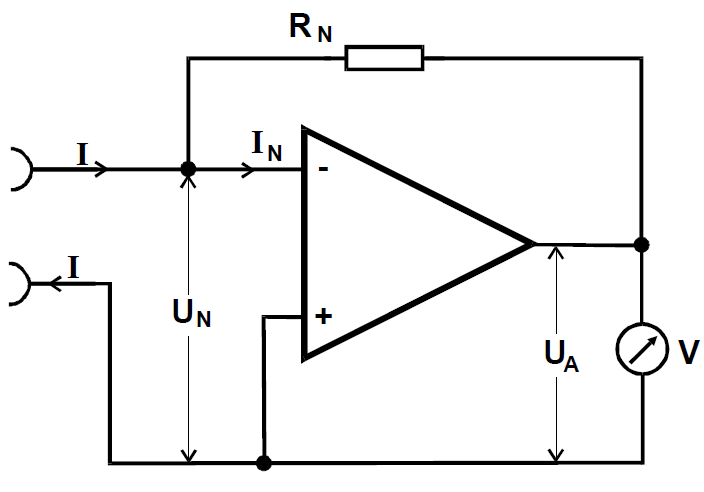
\includegraphics[width=9cm]{images/schaltplan_amperemeter.png}
\caption{Schaltplan eines Amp$\grave{\text{e}}$remeters}
\label{fig:schaltplan_amperemeter}
\end{figure} 












\subsubsection{Logarithmierer und Exponentialgenerator}
Ein Signal proportional zum Logarithmus oder zur Exponentialfunktion kann mit Hilfe eines Bauelement mit exponentieller Kennlinie bewerkstelligt werden, wie in Abbildung \ref{fig:schalplan_explog} dargestellt.

Ein geeignetes Bauteil ist beispielsweise eine Diode bei hinreichend großer Spannung $U$, denn dann gilt
\begin{align}
I=I_0 \exp \left(\frac{e_0}{k_\text{B} T}U\right)
\end{align}
mit der Elementarladung $e_0$, der Boltzmann-Konstante $k_\text{B}$ und der Temperatur $T$. 


\begin{figure}[H]
\centering
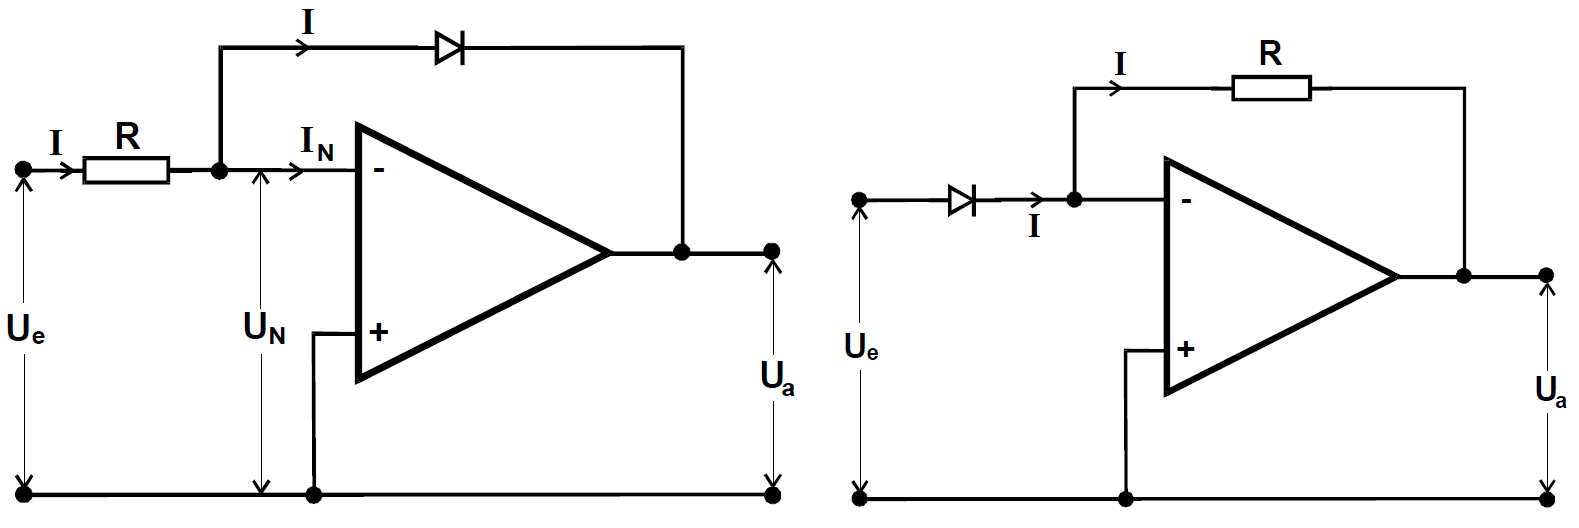
\includegraphics[width=15cm]{images/schaltplan_explog.png}
\caption{Schaltplan eines Logarithmierer (links) und eines Exponentialgenerator (rechts). [1]}
\label{fig:schalplan_explog}
\end{figure}

Es ergibt sich für einen Logarithmierer die Ausgangsspannung 
\begin{align}
U_\text{A}=\frac{k_\text{B}T}{e_0}\ln \left(\frac{U_\text{e}}{I_0 R}\right)
\end{align}
und für einen Exponentialgenerator die Ausgangsspannung
\begin{align}
U_\text{A}=RI_0\exp \left(\frac{e_0}{k_\text{B} T}U_\text{e}\right)\hspace{0.3cm}\text{.}
\end{align}
